%% Requires compilation with XeLaTeX or LuaLaTeX
\documentclass[
  10pt,
  aspectratio=169,
  xcolor={dvipsnames,table,x11names},  % -- To avoid option clash, this seems to load xcolor before theme and thus avoid clash
]{beamer}


% -- Include theme
\makeatletter
\def\input@path{{../GWtheme/}}
\makeatother
\usetheme{GW}


% -- Prevent error from graphicspath
\usepackage{graphicx}
\graphicspath{{./}{../}}


% -- Update GWBar Options -----------------------------------------------------
\UpdateGWBarOptions[% The percent sign here is super important, otherwise Latex thinks we want to access " templatefile", i.e. a space is inserted
    templatefile="../GWtheme/eccentric_template.txt",
    backgroundsignal="none",
    progressbar=false,
]

% -- In particular, you can set templatefile="none" as well to indicate
% -- that no signal shall be used, which speeds up the compilation (nice
% -- if you are still testing around).

% -- To disable use of GWBar entirely, you can use \setbeamertemplate{headline}{}
% -- which just updates the headline definition in which the \gwbar command is used.



% -- This is the recommended way of updating options. You can also do this more
% -- manually by setting the corresponding \gwbar@<some name> commands manually,
% -- but \UpdateGWBarOptions is more straightforward.

% -----------------------------------------------------------------------------


% -- Other stuff
% \pgfdeclareimage[height=0.1\paperheight]{logo}{example-image}

\title[Your Short Title]{Your Presentation}
\subtitle{Your subtitle (if there's one)}
% \author{Your Name \and Another Name}
% \author[Your name (short)]{Your Name}
\author[\MakeUppercase{Your name (short)}]{Your Name \and Another Name}  % For use with \insertshortauthor in footline
\institute{Your Faculty/Department}
\date{Date of Presentation}


% -- Make Berkeley examples work
\usepackage{array}
\usepackage{colortbl}


\renewcommand{\arraystretch}{1.2}
\newcommand{\tableheadrow}{\rowcolor{block title.fg}}
\newcommand{\tableheadcol}[1]{{\bfseries\color{white}#1}}
\AtBeginEnvironment{tabular}{\color{black}}


\begin{document}

{  % -- Brackets required for temporary settings related to titlepage
% \setbeamertemplate{headline}{}  % We do not want GW on here -> done by plain already, also disables footline
\setbeamertemplate{background}{}
\begin{frame}[t, plain, noframenumbering]  % Equivalent to previous line
  \vspace*{-3\baselineskip}%  Adjusts until it fits
  \titlepage
\end{frame}
}


\begin{frame}{Outline}
  \hypersetup{linkcolor=black}
  \tableofcontents[sectionstyle=shaded/show, hideallsubsections]
\end{frame}

\section{Introduction}
  \subsection{Test}

\begin{frame}

\begin{itemize}
  \item Your introduction goes here!
  \item Use \texttt{itemize} to organize your main points.
\end{itemize}

\begin{block}{Examples}
Some examples of commonly used commands and features are included, to help you get started.
\end{block}

\end{frame}

\section{Some \LaTeX{} Examples}

\subsection{Mathematics}

\begin{frame}{Readable Mathematics 42}

Let $X_1, X_2, \ldots, X_n$ be a sequence of independent and identically distributed random variables with $\text{E}[X_i] = \mu$ and $\text{Var}[X_i] = \sigma^2 < \infty$, and let
$$S_n = \frac{X_1 + X_2 + \cdots + X_n}{n}
      = \frac{1}{n}\sum_{i}^{n} X_i$$
denote their mean. Then as $n$ approaches infinity, the random variables $\sqrt{n}(S_n - \mu)$ converge in distribution to a normal $\mathcal{N}(0, \sigma^2)$.

\end{frame}


\subsection{Tables and Figures}

\begin{frame}{Tables and Figures}

\begin{itemize}
\item Use \texttt{tabular} for basic tables --- see Table~\ref{tab:widgets}, for example.
\item You can upload a figure (JPEG, PNG or PDF) using the files menu. 
\item To include it in your document, use the \texttt{includegraphics} command (see the comment below in the source code).
\end{itemize}

\begin{table}
\centering
\begin{tabular}{l r}
\tableheadrow
\tableheadcol{Item} & \tableheadcol{Quantity} \\
\rowcolor{gray!42}
Widgets & 42 \\
\rowcolor{gray!24}
Gadgets & 13
\end{tabular}
\caption{\label{tab:widgets}An example table.}
\end{table}

\end{frame}

\begin{frame}
\frametitle{Figure Example}

Commands to include a figure:

\begin{figure}
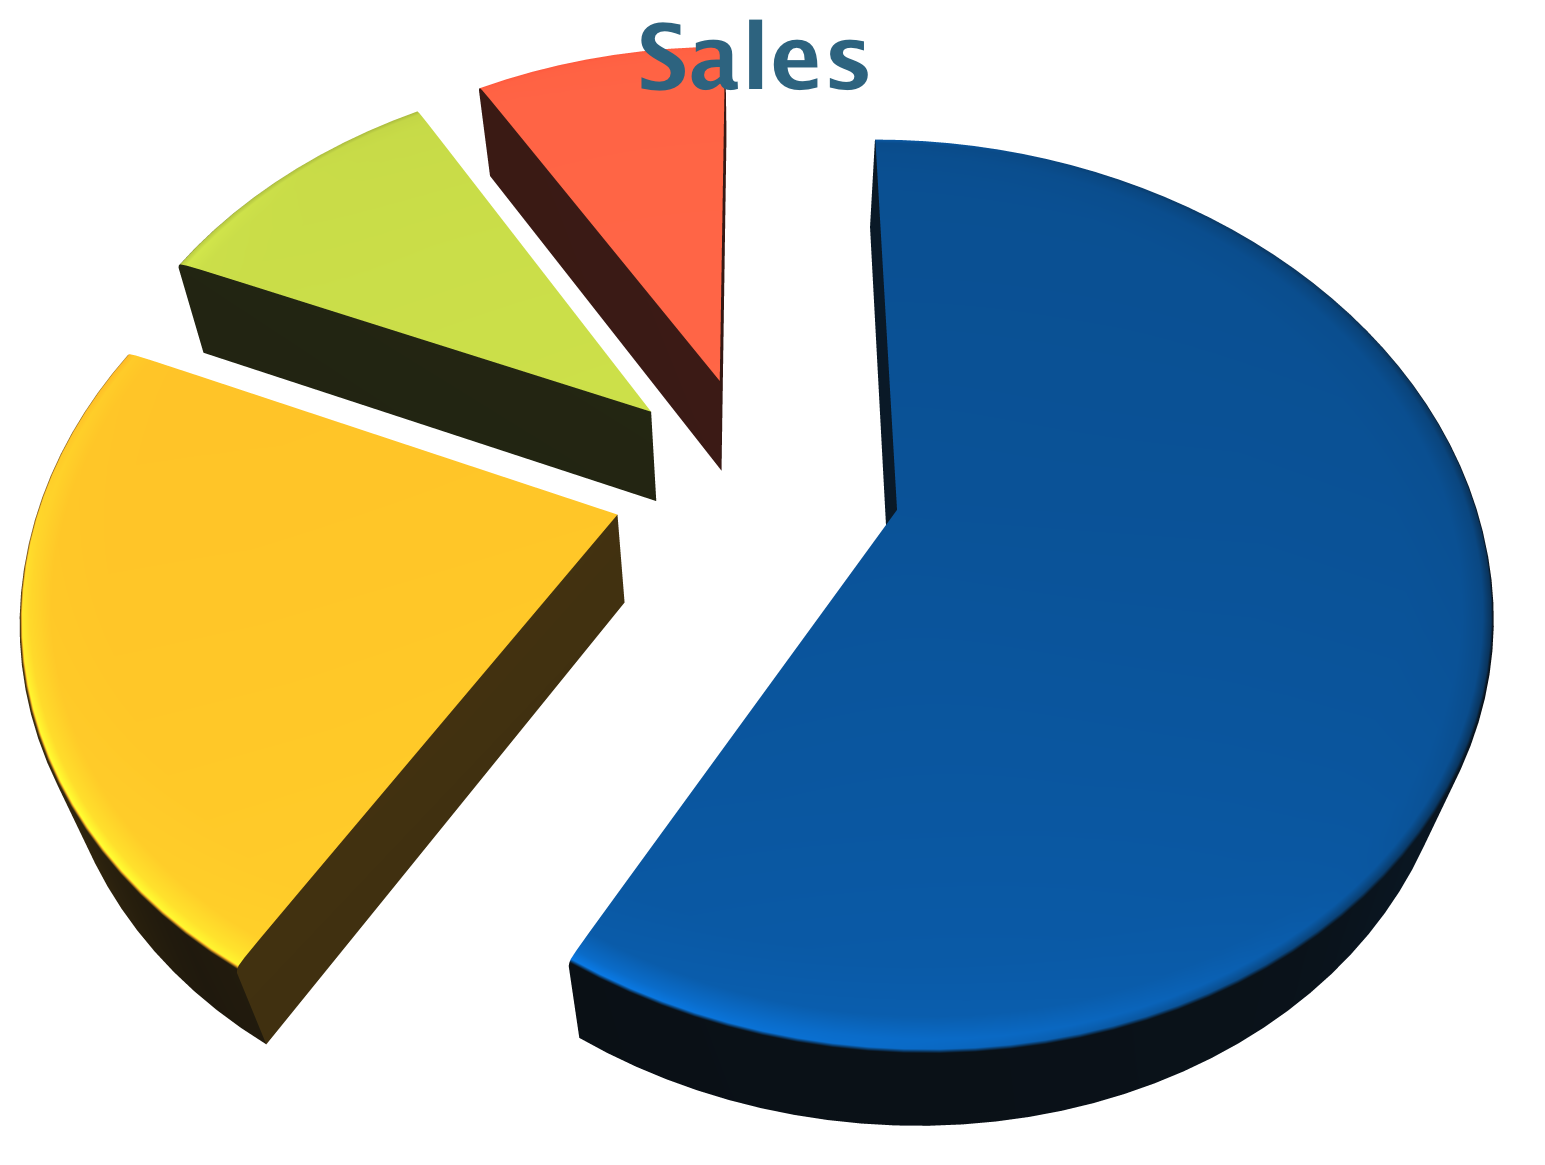
\includegraphics[width=0.4\textwidth]{chart}
\caption{\label{fig:your-figure}Caption goes here.}
\end{figure}
\end{frame}

\begin{frame}
\frametitle{Text in Two Columns}

\begin{columns}[T]

\begin{column}{0.48\textwidth}
\small
Lorem ipsum dolor sit amet, consectetur adipiscing elit. Fusce sit amet massa in dolor pellentesque tempor. Integer nunc. 
\end{column}

\begin{column}{0.48\textwidth}
\begin{itemize}
\item First bullet goes here
  \begin{itemize}
  \item Secondary bullet goes here
    \begin{itemize}
    \item Tertiary bullet goes here
    \end{itemize}
  \end{itemize}
\end{itemize}
\end{column}

\end{columns}
\end{frame}


\appendix  % Frame numbers end at this point

\begin{frame}
\frametitle{Lorem Ipsum}

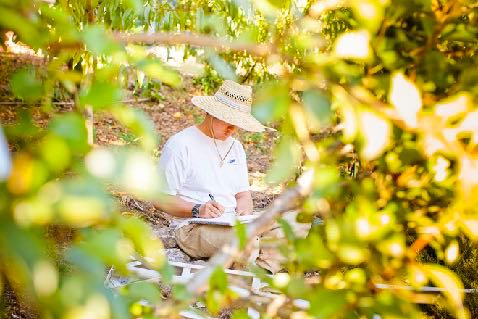
\includegraphics[width=.65\textwidth,height=.5\textheight]{photo}

\end{frame}


\end{document}
